\section{Consuntivazione}

\subsection{Milestones:}
\begin{itemize}
    \item Analisi dei requisiti v1.0.0 (Completa al: 50\%)
    \item Requirements and technology baseline (Completa al: 30\%)
\end{itemize}

\subsection{Attività svolte}


\begin{center}
    \begin{tabularx}{\textwidth}{X l}
        
        \rowcolor{gray!30} \textbf{Attività} & \textbf{stato}\\
        
        \hline

        definizione uc01 & Completato \\
        \rowcolor{gray!10}definizione uc02 & Completato \\
        definizione uc03   & Completato \\
        \rowcolor{gray!10}definizione uc04 & Completato \\
        definizione uc05 & Completato \\
        \rowcolor{gray!10}definizione uc06 & Completato \\
        definizione uc07 & Completato \\
        \rowcolor{gray!10}definizione uc08 & Completato \\
        definizione uc09   & Completato \\
        \rowcolor{gray!10}definizione uc10 & Completato \\
        stesura generale del'analisi dei requisiti & Completato\\
        \rowcolor{gray!10}stesura glossario & Non completato\\
        esternalizzazione del documento di vision & Completato\\
        \rowcolor{gray!10}creazione di un ambiente \textit{github pages} & Parzialmente completato\\
    \end{tabularx}
\end{center}


\begin{table}[h]
    \begin{tabularx}{\linewidth}{X|rrrrrrr}
    \rowcolor{gray!30}& Re & Amm & An & Pro & Prog & Ver & tot \\
    \hline
    Bonavigo Michele      & 0 & 0    & 1,5  & 0 & 0 & 0,1  & 1,6 \\
    \rowcolor{gray!10}Casarotto Mattia      & 0 & 0    & 0,75 & 0 & 0 & 0    & 0,75\\
    Massarenti Alessandro & 0 & 1,75 & 0,25 & 0 & 0 & 4,5  & 6,5 \\
    \rowcolor{gray!10}Peron Samuel          & 4 & 0    & 0    & 0 & 0 & 1,25 & 5,25\\
    Pierobon Luca         & 0 & 0    & 0    & 0 & 0 & 2,35 & 2,35\\
    \rowcolor{gray!10}Romano Davide         & 0 & 0    & 2,55 & 0 & 0 & 0    & 2,55\\
    Zarantonello Giorgio  & 0 & 0    & 0,5  & 0 & 0 & 0    & 0,5 \\
    \hline
                          & 4 & 1,75 & 5,55 & 0 & 0 & 8,2  & 
    \end{tabularx}
    \caption{\label{ruoli-persone}Spartizione dei ruoli e ore svolte durante lo sprint}
\end{table}

\begin{center}
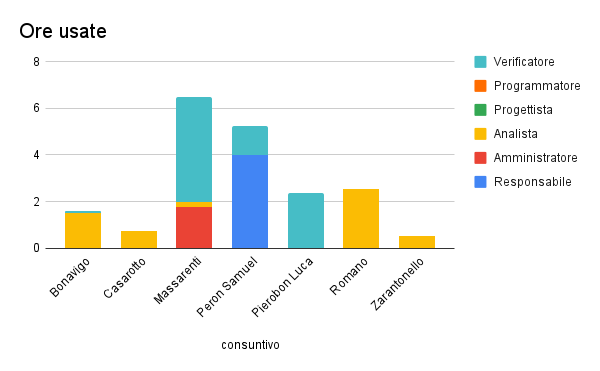
\includegraphics[width=12cm]{img/ore-usate.png}
\end{center}

\begin{table}[h]
    \begin{tabularx}{\linewidth}{X|l|l}
    \rowcolor{gray!30}& Ore & Costo \\
    
    Responsabile & 4 & € 120,00 \\
    \rowcolor{gray!10}Amministratore & 1,75 & € 35,00 \\
    Analista & 5,55 & € 138,75 \\
    \rowcolor{gray!10}Progettista & 0 & € 0,00 \\
    Programmatore & 0 & € 0,00 \\
    \rowcolor{gray!10}Verificatore & 8,2 &€ 123,00 \\
    totale & 19,5 & € 416,75 \\
    \end{tabularx}
    \caption{\label{costi-ruolo}Spartizione dei ruoli e ore svolte durante lo sprint}
\end{table}


Avendo quindi consumeto €416,75\footnote{Si veda tabella \ref{costi-ruolo}} del budget durante questo sprint, rimangono ancora a disposizione €13683,25 per gli sprint rimanenti.
